\chapter{Tezos-specific Offline Design}\label{chap:offline_tezos}
After parsing an assertion contract and transforming it, the resulting AST is passed to the target-specific backend. For this thesis, the platform target is Tezos, with Michelson as the compilation target. This chapter continues to describe the pipeline stages implemented in the Tezos backend, which are shown in \figref{fig:pipeline_backend}. Furthermore, it states the necessary extensions to Michelson and its evaluator to facilitate useful assertions using random generators and assesses several orchestration strategies between the parent and assertion contract code. As a preliminary, the following section gives a short introduction to the Tezos blockchain, the Michelson language and some relevant tools in Tezos' ecosystem.

\section{Introduction to Tezos}\label{sec:tezos}
The Tezos blockchain is presented in its whitepaper as a \enquote{generic and self-amending crypto-ledger} \cite{goodman_tezos_2014}. It uses a proof-of-stake consensus mechanism that is not only used to agree on the current state of its ledger, but also allows its stakeholders to come to a consensus about changes in the economic protocol by participating in a voting process. The changes included in a protocol upgrade, called amendment, can influence i.a. which transactions are valid on the blockchain, the payment system or even the voting process itself without risking a fork of the blockchain. Everyone owning the cryptocurrency of Tezos, called Tez, is considered a stakeholder and can participate in the consensus mechanism. The whitepaper compares the self-amending protocol of Tezos to a game created by Philosopher Peter Suber called ``Nomic'', whose set of rules are subjected to a democratic voting system \cite{nomic}. Similar concepts can also be found in modern pop culture, such as the virtual sports league ``Blaseball'' \cite{blaseball} that became popular during the COVID-19 pandemic.

In addition to user accounts associated with a public key, Tezos supports smart contracts, which are written in the built-in language Michelson. Tezos' transaction fee system is similar to that of Ethereum \cite{wood_ethereum_2021} - it is gas-instrumented and besides a base fee, every operation and byte of storage during contract execution has to be paid for. However, Tezos imposes a hard cap on the amount of gas that can be consumed per operation (including internal transactions) \cite{tezos_docs}\cite{morley_repo}, whereas Ethereum limits the gas quota only in respect to blocks \cite{wood_ethereum_2021}.\\
Tezos is written in the multi-paradigm programming language OCaml \cite{ocaml_doc}. Compiling the its source code yields five essential binaries: the node, baker, endorser, accuser and client. The node is the entity that connects to the peer-to-peer network and keeps a copy of the chain. Bakers are responsible for producing new blocks, the endorsers for validating new blocks and the accusers to call out bakers or endorsers which double-sign or -endorse. The client provides a command line interface to interact with the local node through remote procedure calls (RPC).

\subsection{Proof-of-stake in Tezos}
In Tezos, contracts that staked a minimum amount of tokens, called a roll, can participate in the consensus mechanism and can either have the role of a baker or endorser. Contracts who don't own enough tokens or infrastructure to participate directly can delegate their baking and endorsing rights to other contracts. The rights are determined and assigned at the beginning of each cycle, which consists of a specified number of blocks. For baking, a random roll is selected for each block level and the rights are assigned to its owner. The block produced by that baker is endorsed by a fixed number of endorsers (currently 32 in protocol 008 Edo), which also have been assigned endorsing rights for this block level by a random selection of rolls. Since participants can stake more than one roll, an endorser may be assigned several endorsement slots at the same block level. \\
As an incentive for active participation in the consensus algorithm, delegates (and also delegators) receive rewards in form of tokens. However, if accusers detect double-baking or -endorsement, the delegate is penalized by burning (i.e., destroying) their security deposit. \cite{tezos_docs}

\subsection{Michelson}
Michelson is a lower-level, stack-based language with strict type-checking and supports primitive data types, like integers or strings, as well as high-level data structures such as list, maps and sum types \cite{tezos_docs}. The type system reduces the occurrence of runtime errors and ensures that only well-typed contracts are originated on the blockchain. \\
The concrete syntax of Michelson is called Micheline. A program is represented in Micheline nodes, which can be one of the following constructs:
\begin{itemize}
\item A constant of type integer (in decimal notation)
\item A constant of type string
\item A byte sequence in hexadecimal notation
\item An application of a language primitive to a sequence of nodes
\item A sequence of nodes
\end{itemize}
For documentation, readability and additional type constraints, Michelson and Micheline also offer three types of annotations - type, variable and field or constructor annotations, which are labelled with a unique special character in Micheline. The toplevel structure of a smart contract consists of a sequence of the three primitives \texttt{parameter, storage} and \texttt{code}, declaring the type of the input parameter, the storage type and the actual program code. The full grammar of Micheline and Michelson can be found in the Tezos developer resources \cite{tezos_docs}.

\subsubsection{Entrypoints}
 Unlike the contracts shown so far, which were expressed with the syntax of Ethereum's contract language Solidity \cite{solidity_docs}, Michelson doesn't have a concept of named functions with individual input parameter types. Instead of named functions, Michelson programs can have separate entrypoints by taking a disjunctive type as input parameter and optionally tagging the type constructors with a "function" name. The disjunctive type is built by nesting the \texttt{or} type, which has the constructors \texttt{left} and \texttt{right}. Assume we want to implement the contract from \lstref{lst:prime} in Michelson and add another function to it, which expects a string parameter. Omitting the actual program, the contract type declaration looks as follows:
\begin{lstlisting}[language=Michelson, numbers=none, caption=Michelson contract with two entrypoints]
parameter (or (int %isPrime) (string %isUpper));
storage unit;
code {
  ...
  IF_LEFT { ... (* then *)}
          { ... (* else *)}
}
\end{lstlisting}
The input type declared in the primitive application \texttt{parameter} accepts input of either type \texttt{left int}, or \texttt{right string}. By adding the field annotations \texttt{isPrime} and \texttt{isUpper}, the entrypoints are given tags and can be called explicitly by an external transaction. In that case, parameters of type \texttt{int} or \texttt{string} are accepted and the value is automatically wrapped into the respective constructors. Furthermore, it's possible to declare a \texttt{default} entrypoint, which is called when no explicit tag is specified. By default, the default entrypoint is assigned to the root of the parameter type. \cite{tezos_docs}

\subsection{Developer tools in the Tezos ecosystem}
This section describes some relevant tools and projects for developers that are part of Tezos' ecosystem.

\subsubsection{Tezos Libraries}
Tezos' executables and libraries are developed in the programming language OCaml and are available on through OCaml's package manager \texttt{opam} \cite{tezos_opam}. The protocol libraries of every version are released separately, thus any projects can be built on the protocol of choice. Important libraries that were used in the development of the offline toolchain are the Micheline library providing the internal abstract syntax tree (AST) and parser of the Michelson language, as well as the protocol specific libraries containing i.a. the type checker. Additionally, the client libraries are used to retrieve any needed information from the node or blockchain via RPCs.

\subsubsection{Testing tools}
Before a new protocol is proposed to the Tezos network, it has to be thoroughly tested with system, integration and regression tests. This requires a sandboxed network to simulate the real peer-to-peer network, such that also interactions between the actors of the blockchain can be tested. Tezos' development environment provides two testing frameworks for this:
\begin{itemize}
\item[\textbf{Flextesa}] With Flextesa (Flexible network sandboxes)\cite{tezos_docs} one can configure and run a small, fully functional sandboxed test network including nodes, bakers, endorsers and accusers. Accounts can be instantiated and used to send or receive funds. Configurable are, for instance, the size of the network, the time between blocks or enabling generation of random network traffic. Networks may either be fully autonomous, baking blocks automatically, or require manual baking of blocks. It also supports interactive sessions, where the tester can interact with the blockchain using the Tezos client. Flextesa's typical use-cases are interactive testing scenarios like double-baking, the voting process or protocol amendments. The Tezos repository already provides ready-to-use scenarios for accusations. Besides testing shell or protocol code, Flextesa can also be used to test smart contracts.
\item[\textbf{Tezt}] The Tezt framework \cite{tezos_docs} is newer than Flextesa and planned as its replacement. It launches the Tezos binaries as external processes to build a sandboxed test network of configurable size. Its main advantages over Flextesa are simplicity, better usability and extendibility and better performance due to the use of an event system instead of polling the node.
\end{itemize}

\subsubsection{High-level languages}
Michelson is a compilation target for various high-level languages that provide a more user-friendly and intuitive way of writing smart contracts. Additionally, some of them come with development environments and testing or verification tools. The following list comprises of the three most prominent languages that compile to Michelson:
\begin{itemize}
\item[\textbf{Liquidity}] \cite{liquidity} is a language with an OCaml-like syntax, which allows using local variables instead of stack manipulations. Its module system can be used to write reusable contract code or libraries. Besides an optimizing compiler, the project also includes a decompiler to compile Michelson programs to Liquidity.
\item[\textbf{SmartPy}] \cite{smartpy} is a language available through a Python library and lets developers write contracts and tests using Python syntax and structures (such as classes). Its developer suite includes i.a. a compiler, a simulation engine for testing contracts and an online editor.
\item [\textbf{fi}] 's \cite{fi} syntax is similar to JavaScript or Ethereum's contract language Solidity. It also provides an online editor and a simulator to test against the compiled contracts. However, it seems extensions to Michelson introduced by newer protocol versions are not supported yet.
\end{itemize}

\section{Extensions to Michelson}
The way Michelson is interpreted is purely functional; it takes the current stack and an operation and builds a return stack from the initial one, without causing any side effects \cite{tezos_docs}. The recursive Michelson interpreter is defined as as a list of rules comprising of all possible inputs, i.e. program and stack types, and the respective output stack type of the computation if a rule applies. Each rule is of the following form: 
\begin{lstlisting}[caption=Rules form in the Michelson interpreter \cite{tezos_docs}, language=, numbers=none, label=lst:rules]
> (syntax pattern) / (initial stack pattern)  =>  (result stack pattern)
    iff (conditions)
    where (recursions)
    and (more recursions)
\end{lstlisting}
For each valid program and initial stack exactly one rule matches (given that any extra conditions over values on the stack, stated after the \texttt{iff} keyword are true) \cite{tezos_docs}. If the result depends on the results of other program interpretations (given after the keywords \texttt{iff, where, and} in rule form), the rule only applies if these partial results also match the respective intermediate result stack patterns.\\
In addition, there exists a typing rule for each syntax construct that restricts the valid input stacks. The typing rules use the meta variables \texttt{'a} for type and \texttt{'A} for stack type variables in order to express consistency within the program (not polymorphism). These rules are given in the following form:
\begin{lstlisting}[caption=Form of typing rules in Michelson's specification \cite{tezos_docs}, language=, numbers=none, label=lst:type_rules]
(syntax pattern)
:: (type of stack before) -> (type of stack after) [rule-name]
   iff (premises)
\end{lstlisting}
The type notations, as well as syntax and stack patterns are listed in \cite{tezos_docs}.\\

From the given formulas and assertion examples so far, one can derive a set of necessary instructions that need be be present in the target language. The following subsections list the instructions which have to be added to Michelson's instruction set, specify their selection and typing rules and describe how they can be implemented in the interpreter. These do not necessarily include high level instructions, like \texttt{sqrt} from \eqref{eq:prime}, that can be reproduced by using lower level instructions. For these purposes, a later iteration of the syntax will provide the feature of user-defined functions.

\subsection{Random}
A vital instruction that cannot be expressed with Michelson's current instruction set (state of protocol 008 Edo \cite{tezos_docs}) is the generation of a random value of certain types. Since smart contracts need to be deterministic, s.t. the network can reach a consensus about the state of the ledger \cite{chatterjee_probabilistic_2019}, the prevalent workarounds for generating pseudo-random numbers cannot be used for assertion checking. Distributed assertion checking explicitly requires as many validators as possible to generate a unique value, whereas common schemes for randomness, like oracles or using block attributes as seeds \cite{chatterjee_probabilistic_2019}, will provide the same values for all validators.\\
\lstref{lst:rand_type} specifies the selection and typing rule of a new instruction \texttt{rand}, which consumes an offset and a positive range from the stack and pushes a randomly generated integer to the top. This instruction, of course, can also be provided for other data types, such as \texttt{nat}, \texttt{string} or \texttt{mutez}.
\lstset{upquote=true}
\begin{lstlisting}[caption=Selection and typing rules of the integer \texttt{rand} instruction, language=, numbers=none, label=lst:rand_type]
:: int : nat: 'A -> int : 'A
> RAND/ offset : range : S  => int : S
\end{lstlisting}

Within the Michelson interpreter, the selection of rules is implemented as a huge match case \cite{tezos_repo}. If the rule for \texttt{rand} applies, the respective computation in OCaml could look as drafted in \lstref{lst:rand_impl}.
\begin{lstlisting}[caption=Simplified evaluation of \texttt{rand} in the Michelson interpreter, language=, label=lst:rand_impl]
match (instruction, stack) with
...
| (Rand (offset, (range, rest))) -> 
   Random.self_init;
   let rand_int = offset + Random.int(range) in
   return (rand_int, rest)  (* Resulting stack *)
\end{lstlisting}

\subsection{Nth}
An exception for not adding higher level instructions may be the more fundamental operation \texttt{nth} for accessing list elements, as it is used (sometimes more than once, ref. \eqref{eq:sorted_v2}) in many use cases. Adding an own predefined primitive for this reduces the origination costs of the assertion contract, given that its equivalent in the current instruction set requires the compiler to generate a workaround using iteration, for instance a loop or list iterator. As a first approximation, appendix \ref{apx:nth} shows a potential implementation of \texttt{nth} in Liquidity (\lstref{lst:nth_liq}) using a loop, and how the respective Michelson code looks like after compiling the contract with the Liquidity compiler (\lstref{lst:nth_tz}). \\
In case the \texttt{nth} is added as a predefined primitive to Michelson for the type \texttt{'a list}, its selection and typing rules are specified as follows:
\begin{lstlisting}[caption=Selection and type rule of the list \texttt{nth} instruction, language=, label=lst:nth_type]
:: (list 'a) : nat : 'A -> option 'a : 'A
> NTH / l : index : S  =>  Some 'a: S
     iff index is within bounds
> NTH / l : index : S  =>  None 'a: S
     iff index is out of  bounds
\end{lstlisting}
As Michelson lists are represented with OCamls list type within the VM \cite{tezos_repo}, the computation for \texttt{nth} could look as shown in \lstref{lst:nth_impl}.
\begin{lstlisting}[caption=Simplified evaluation of \texttt{nth} in the Michelson interpreter, language=, label=lst:nth_impl]
match (instruction, stack) with
...
| (Nth ({elements = []; _}, (_, rest))) ->
  return ((None, rest)
| (Nth ({elements = es; length}, (index, rest))) ->
  let l_length = of_int length in
  if index <= l_length
    then return (Some (List.nth es index), rest)
    else return (None, rest)
\end{lstlisting}
\lstset{upquote=false}

\section{Orchestration of contract and assertions}
So far, the assertion and parent contract have been considered separately. However, on the blockchain they have to be orchestrated, s.t. the bakers and validators execute the assertion before the actual contract code. The orchestration does not only include the linking of assertion and contract code, but also a mechanism to execute an assertion $n$ times depending on the domain space that needs to be checked. There are basically two approaches - the assertion and contract code can be assembled into a single monolithic contract, or they can be originated separately as standalone contracts. As the strategy has an impact on the compilation process and output, it has to be determined in advance which of the two should be implemented and how.

\subsection{Approach 1: Monolithic contract}
In the monolithic approach, a new contract is built using both the assertion and parent code as input. As is outlined in \figref{fig:monolithic_orchestration_basic}, the assertions can either be appended to the original contract as separate entrypoints or by prepending them to the code of the respective entrypoint. This tightly couples and unites the code in one self-contained unit.
\begin{figure}[!htb]
\subfloat[Appending assertions as separate entrypoints]{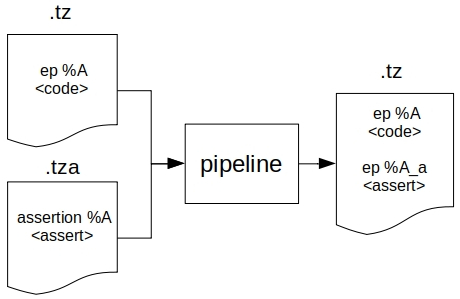
\includegraphics[width=0.5\textwidth]{figures/4-offline_tezos/monolithic_ep.jpg}}
\quad
\subfloat[Inserting the assertion code into the original entrypoint]{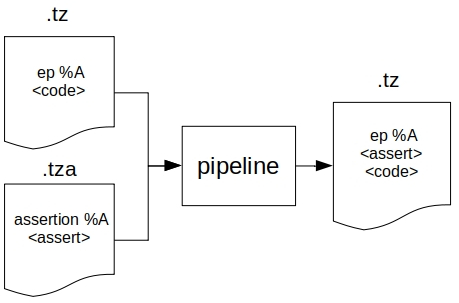
\includegraphics[width=0.5\textwidth]{figures/4-offline_tezos/monolithic_insert.jpg}}
\caption{Approaches for assembling a monolithic contract}
\label{fig:monolithic_orchestration_basic}
\end{figure}
While the link between assertion and contract code is already given in a), the entrypoint and assertions in b) still need to be coupled, as it is not inherent which entrypoint represents a normal and which the respective assertion. For this reason, assertion entrypoints need to have fixed name pattern, s.t. it is derivable from the original entrypoint. As a proposal, the tag of the assertion is the tag of its parent entrypoint suffixed with a \texttt{\_a}, e.g. \texttt{A\_a} for entrypoint \texttt{A}. The baker can then execute the contract normally by calling the original entrypoint and prompt the validators to execute the assertion separately. \\
Both approaches, however, do not yet provide any means to have validators execute the assertions $n$ times. Since only the contract itself knows how to calculate $n$ (as per the range(s) of the random generator(s)), it cannot be passed to the validators as a parameter to the validation request. Instead, the contract itself needs a test run manager which handles this. A test run manager can either be implemented as another entrypoint, say \texttt{A\_m}, which then calls \texttt{A\_a} (or \texttt{A} in case of a)) $n$ times as an internal transaction. Another possibility is to create a separate manager contract that acts as a proxy, contains the manager code and internally calls the monolithic contract. This solution is a hybrid of the monolithic and modular approach. The section covering the modular approach describes in more detail how it is implemented.\\
It's important to realize that neither baker nor validators can differentiate between entrypoints that have an associated assertion and those that do not. In order to avoid transaction failures caused by calling assertions that do not exist, the compiler has to add dummy managers for empty assertions that call the actual contract code immediately.\\
% Description figures
% -> txa special transaction type
% managers use internal transactions to call contract n times
% depending on protocol, validators use normal tx or another special tx type
% req message needs to contain the derived name of the assertion ep -> derivation needs to be part of the "assertion mode". is this possible?
% veto message: the txa op hash it refers to, an instance of a counterexample (not yet clear how this looks like)

\begin{figure}[h]
\centering
  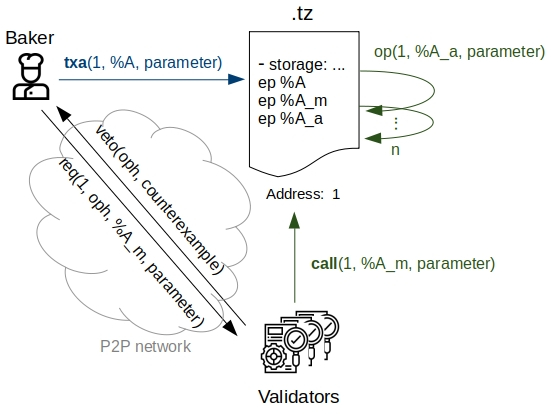
\includegraphics[width=0.7\textwidth]{figures/4-offline_tezos/interaction_monolithic.jpg}
	\caption{Interaction with a monolithic contract}
	\label{fig:interaction_monolithic}
\end{figure}

\begin{figure}[h]
\centering
  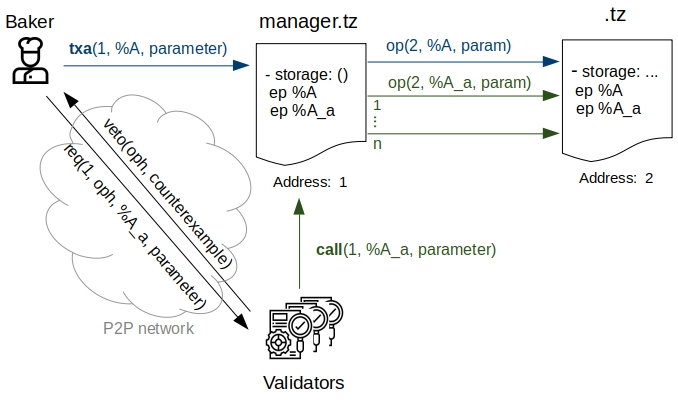
\includegraphics[width=0.8\textwidth]{figures/4-offline_tezos/interaction_monolithic_managertz.jpg}
	\caption{Interaction with a manager and monolithic contract}
	\label{fig:interaction_monolithic_managertz}
\end{figure}

\subsubsection{Evaluation}
Generell:
- parent code has to be modified
	+ show code example
	+ decompilation necessary
	+ compilation is more complex
- doesn't work if the parent code is already originated
- inflexible -> tightly coupled code
	+ if the assertion code changes, the whole contract has to be reoriginated

ep assert + ep manager
+ baker can call basic ep; validators call manager
	-> cost efficient; contract is only executed once
- only works with explicit ep -> parameter types!
- complex compilation (1-2 eps per ep more)
- readability

no ep assert + ep manager
- contract code is also executed n times
- only works with explicit ep -> parameter types!
+ bypassing assertion not possible!
+ less eps more readable? (aber nur bisschen)

ep assert + contract manager
+ less complex compilation -> just copy assertion code before the actual code (less entrypoint handling)
+ if manager also has eps A and A\_m, the code and assertions can also be called separately
+ modularity -> readability, a bit more flexibility (if manager code changes)
- \^ even more eps -> 2-3 eps more
- more boilerplate, more origination costs

no ep assert + contract manager
- contract code is also executed n times
+ bypassing assertion not possible!
+ less complex compilation -> just copy assertion code before the actual code (less entrypoint handling)
+ modularity


what happens to calls to default?






\begin{itemize}
\item Assertions are appended to the parent as separate entry points
\item Parent contract has to be modified (parameter type \& addendum)
\item Problems/Drawbacks:
	\begin{itemize}
	\item entrypoint names necessary - otherwise no unambiguous assignment
	\item parameter types of original ep \& assertion ep are different
	\item e.g. \%A and \%A\_a cannot be called with the same parameter (if not called explicitly; ref. \ref{lst:mono_unnamed} line 24, 25.)
	\item Possible solution:
		\begin{itemize}
		\item all eps in the parent and assertion contract need to have a \%name \verb|->| calling both eps explicitly allows using the same parameter (ASAIK) ; ref. \ref{lst:mono} line 24, 25.
		\item Assign dummy names if none are given - effort?
		\item what to do with calls to \%default?
			\begin{itemize}
			\item Baker would need to
			\item 1) look up entrypoints of contract 
			\item 2) check which type matches \& find out the ep name
			\item 3) derive assertion ep name from that
			\end{itemize}
		\item how to assign entry points given without names in .tza to their respective parent eps? \ref{lst:mono_unnamed} line 10, 11.
		\end{itemize}
	\end{itemize}
\item EP names of the assertion code need to have a fixed pattern, s.t. the bakers know how to call them
\item Similarly to strategy 1, there probably needs to be "empty" assertion code for normal eps
\end{itemize}

%\ref{fig:separate_contract_v2}:
%\begin{figure}[h]
%	\centering
%  \includegraphics[width=\textwidth]{assembly_monolith}
%	\caption{Interaction with a monolithic contract}
%	\label{fig:monolithic_contract}
%\end{figure}

%\lstinputlisting[label=lst:mono, caption=Monolithic assembly w/ ep names, numbers=left]{monolithic.tz}
%\lstinputlisting[label=lst:mono_unnamed, caption=Monolithic assembly w/o ep names, numbers=left]{monolithic_unnamed.tz}

\subsection{Approach 2: }


\section{Backend of the pipeline}
The Tezos backend of the pipeline comprises of the three stages semantic check, type check and compilation. During the semantic check, the common AST is cast to a Tezos-specific AST type. If the assertion contains any data types or operations not supported in Michelson, the assertion contract is rejected. Since the subsequent stages are less straight forward, they are explained in more detail in the following.
\begin{figure}[h]
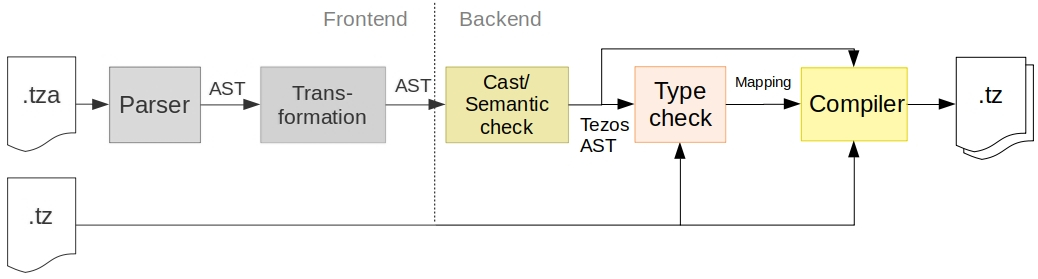
\includegraphics[width=\linewidth]{figures/4-offline_tezos/pipeline_backend}
\caption{The stages of Tezos-specific backend of the compilation pipeline}
\label{fig:pipeline_backend}
\end{figure}

\subsection{Type check}
The task of the type checker is to map the assertions from the given file to the respective entrypoints of the parent contract. To this end, the parameter types have to be compared and matched against each other in order to find a correct assignment. The type checker either reads the code of the parent contract from a given file or retrieves the code from a given address on the blockchain. It must be ensured that the created mapping is injective and unambiguous, i.e., each assertion matches exactly one entrypoint and no entrypoint is covered by more than one assertion.\\
As explained in \secref{sec:tezos}, entrypoints can be selected by calling the default entrypoint and wrapping the parameter into the respective union constructors. Alternatively, they can be called explicitly using their tag and passing the parameter as raw value. The same applies for the assertions - by omitting the tag, the parameter type must be declared in respect to the default entrypoint type. If the assertion states an explicit tag, it may declare the raw parameter type. The tags do not necessarily have to be identical with the tags of the parent contract; in some cases, they may be chosen differently for documentation or for readability purposes. However, the tags can and should be used to resolve ambiguity in the mapping between assertions and entrypoints, that is if several entrypoints share the same input type. Ambiguity can also be caused by the fact that entrypoints can be sub-entrypoints of others, thus assertions overlap if a separate assertion is declared for both super- and sub-entrypoint. This is resolved by detecting overlapping assertions during the type check and rejecting assertion contracts where appropriate. \\
As an exemplification, consider a Michelson contract with five entrypoints (including the default entrypoint):
\begin{lstlisting}[numbers=none, language=Michelson]
parameter (or (int %A) (or %BC (int %B) (int %C)))
\end{lstlisting}
The following assertion contract for the given PC contains some valid and some invalid assertions:
\begin{lstlisting}[language=Assertion]
(assertion %A (i : int) ...)			 		  (* valid *)
(assertion %D (i : int) ...)			 		  (* invalid *)
(assertion (right (left (i : int)) ...)	(* valid *)
(assertion %BC (x : (or int int)) ...)	(* invalid *)
\end{lstlisting}
Due to its tag, the fist assertion can be assigned unambiguously to entrypoint A, whereas for the second it is not apparent whether it should be assigned to entrypoint B or C. Since the tag is omitted in the third assertion, the parameter type is given in respect to the default entrypoint and is assigned to B. The last assertion is invalid because it is overlapping with the previous assertion, which was already assigned to entrypoint B.

\subsection{Compiler}
The transformed and type checked assertion AST needs to be retargeted to Michelson code. 

\draft{}
\begin{itemize}
\item Orchestration strategies
	\begin{itemize}
	\item monolithic vs. modular
	\item advantages/disadvantages
	\item \# validators in Tezos \& how to have them run n test runs
	\item security mechanism? (prevent ``dodging'' assertions)
	\end{itemize}
\item Compilation strategies (direct vs. IR)
\end{itemize}

\section{Misc}
\todo{Aspects/questions I don't know yet if or where to put it}
\begin{itemize}
\item Tezos specific costs analysis of chosen orchestration strategy -> PROBLEM: high n might reach operation gas limit?
\item How can bakers differentiate between transactions to ”normal” SC and SCs with assertions?
\item Representation of counterexamples; how to verify them?
\item Basic approach for proofs?
\item Usage pipeline
\end{itemize}


%- Vorschlag von HA: geht so nur für counterexamples.
%- Case Proof-modus: some approval message has to be send actively if no assertion failed.%
%	-> check if transaction fails? würde so ein mechanismus gehen? call case contracts n times. nach n times wird contract aber nicht aufgerufen
%	-> oder: case contracts callen parent wenn property check successful; nicht möglich, da dann manager contract nichts davon weiß

 